%%%%%%%%%%%%%%%%%%%%%%%%%%%%%%%%%%%%%%%%%%%%%%%%%%%%%%%%%%%% 
% This is the official template for theses and seminar papers from the Chair for Information Systems for Sustainable Society (IS3) at the University of Cologne

%
%PREAMBLE
%%%%%%%%%%%%%%%%%%%%%%%%%%%%%%%%%%%%%%%%%%%%%%%%%%%%%%%%%%%%%

\documentclass[a4paper, 12pt]{article}
\usepackage[utf8]{inputenc}
\usepackage[T1]{fontenc}
\usepackage{graphicx}
\usepackage{longtable}
\usepackage{hyperref}
\usepackage{caption}
\usepackage{float}
\usepackage{psl-cover}


% set margins for double-sided printing
\usepackage[left=1cm, right=2.5cm, top=2.5cm, bottom=3cm, bindingoffset=1.5cm, head=15pt]{geometry} 
\usepackage{setspace}
\onehalfspacing
% set headers
\usepackage{fancyhdr}
\pagestyle{fancy}
\fancyhead{}
\fancyfoot{}
\fancyhead[LE,RO]{\textsl{\leftmark}}
\fancyhead[RE,LO]{\thesisauthor}
\fancyfoot[C]{ \\
\thepage}
\renewcommand{\headrulewidth}{0.4pt}
\renewcommand{\footrulewidth}{0.4pt}


% set APA citation style
\usepackage{apacite}
\usepackage[numbib,notlof,notlot,nottoc]{tocbibind}
\pagenumbering{gobble}

%%%%%%%%%%%%%%%%%%%%%%%%%%%%%%%%%%%%%%%%%%%%%%%%%%%%%%%%%%%%%
%THESIS Parameters 
%%%%%%%%%%%%%%%%%%%%%%%%%%%%%%%%%%%%%%%%%%%%%%%%%%%%%%%%%%%%%

\title{AVANCEMENT DE THÈSE
- Validation de 1ère année -
\\
Analyse des mouvements et gestes des piétons via caméra embarquée pour la prédiction de leurs intentions}

%%%%%%%%%%%%%%%%%%%%%%%%%%%%%%%%%%%%%%%%%%%%%%%%%%%%%%%%%%%%%
%DOCUMENT
%%%%%%%%%%%%%%%%%%%%%%%%%%%%%%%%%%%%%%%%%%%%%%%%%%%%%%%%%%%%%

\begin{document}



\author{Joseph Gesnouin}
\date{X Avril 2020}
\jurymember{5}{Fabien Moutarde}{Professeur, Mines ParisTech}{Directeur de thèse}
\jurymember{4}{Bogdan Stanciulescu}{Maître de conférences, Mines ParisTech}{Maitre de thèse}
\jurymember{3}{Steve Pechberti}{Ingénieur de recherche, Vedecom}{Encadrant industriel}

\jurymember{2}{Examinateur 2}{Titre}{Jury}
\jurymember{1}{Examinateur 1}{Titre}{Jury}

%% commandes avec des valeurs par défaut non nulles
%%\institute{nom de l’organisme d’accueil PSL}
\doctoralschool{Ingénierie des Systèmes, Matériaux, Mécanique, Energétique}{621}
\specialty{Informatique temps réel, robotique et automatique.}


\maketitle{}
%%%%%%%%%%%%%%%%%%%%%%%%%%%%%%%%%%%%%%%%%%%%%%%%%%%%%%%%%%%%%
%TITLE PAGE (Pre-defined, just change parameters above)
%%%%%%%%%%%%%%%%%%%%%%%%%%%%%%%%%%%%%%%%%%%%%%%%%%%%%%%%%%%%%
%\input{Template/Title.tex}

%\newpage
%\thispagestyle{empty}
%\strut
%\markboth{}{}
%\newpage

%%%%%%%%%%%%%%%%%%%%%%%%%%%%%%%%%%%%%%%%%%%%%%%%%%%%%%%%%%%%%
%Résumé
%%%%%%%%%%%%%%%%%%%%%%%%%%%%%%%%%%%%%%%%%%%%%%%%%%%%%%%%%%%%%
%
\vspace*{2.5cm}
\noindent\rule[2pt]{\textwidth}{0.5pt}\\
{\textbf{Résumé ---}}
Dans le cadre d’un pivot stratégique d’une entreprise de télécommunication à une entreprise numérique, l’analyse des données récupérées sur les équipements de l’univers résidentiel client permet l’analyse et l’amélioration de la qualité des services Orange. Directement rattaché à l’entité Groupe, le département DAQE (Data Analytics and Qs Enablers) fournit aux domaines d'activité stratégique des moyens de collecte et d’analyse des données des équipements maison. Durant mon apprentissage au sein de ce service, j’ai eu l’opportunité de comprendre l’ensemble de la chaîne de collecte et d’analyse des données à l'aide de technologies Big Data Orange, de mettre en pratique mes savoirs et techniques pour comprendre un environnement complexe et y développer de nouvelles briques de calcul. Pour finir, de nombreuses missions de veilles technologiques et de formations m’ont permis d’apprendre de nouvelles notions et des compétences de communication et d’organisation nécessaires au métier de data scientist.


{\textbf{Mots clés :}}
Data Mining, Chaine de collecte, Big Data, Analyse factorielle, Réseaux bayesiens, Inférence Causale, Apprentissage supervisé, Asymétrie, Livebox, Décodeur TV, Satisfaction Client, QoS.
\\
\noindent\rule[2pt]{\textwidth}{0.5pt}
\begin{center}
  Centre Universitaire des Saints-Pères, Université Paris Descartes \\
  45 Rue des Saints-Pères\\
  75006 Paris
\end{center}




%\newpage
%\thispagestyle{empty}
%\strut
%\markboth{}{}
%\newpage
%%%%%%%%%%%%%%%%%%%%%%%%%%%%%%%%%%%%%%%%%%%%%%%%%%%%%%%%%%%%%
%Confidentialité
%%%%%%%%%%%%%%%%%%%%%%%%%%%%%%%%%%%%%%%%%%%%%%%%%%%%%%%%%%%%%
%\clearpage
\section*{Note de confidentialité}
\label{sec:SOOA}

\vspace{1cm}
Ce document et son contenu sont de la propriété d’ORANGE. Aucun droit de propriété intellectuelle n’est accordé par la communication du présent document ou de son contenu. Ce document ne doit pas être reproduit ou communiqué à un tiers sans l’autorisation écrite d’ORANGE. Ce document et son contenu ne doivent pas être utilisés à d’autres fins que celles qui sont autorisées.
\vspace{1cm}

\textbf{\thesisauthor{}} 

\vspace{0.5cm}
\noindent
Guyancourt, le 10.06.2019


%\newpage
%\thispagestyle{empty}
%\strut
%\markboth{}{}
%\newpage
%%%%%%%%%%%%%%%%%%%%%%%%%%%%%%%%%%%%%%%%%%%%%%%%%%%%%%%%%%%%%
%Remerciements
%%%%%%%%%%%%%%%%%%%%%%%%%%%%%%%%%%%%%%%%%%%%%%%%%%%%%%%%%%%%%
%\clearpage
\section*{Remerciements}
\label{sec:remerciements}


\vspace{0.5cm}



\vspace{0.5cm}

\vspace{0.5cm}


\vspace{0.5cm}


\newpage
\thispagestyle{empty}
\strut
\markboth{}{}
\newpage

\vspace{0.5cm}


\vspace{0.5cm}


\vspace{0.5cm}

\vspace{3cm}
\noindent
\textbf{Joseph} 

\newpage
\thispagestyle{empty}
\strut
\markboth{}{}


%\thispagestyle{empty}
%\strut
%\markboth{}{}
%\clearpage
%\vspace*{\fill}
%\thispagestyle{empty} % optional -- suppress showing of page number
%\begin{quotation}
%\em % optional -- to switch to emphasis (italics) mode
%\medskip
%%\raggedleft
%"Je crois que la science\\ avec conscience et sans orgueil est le seul outil d'émancipation personnelle en premier lieu, collégiale sinon collective en second lieu" - Jean-Yves G.\\
%D'après Rabelais, Elysée Reclus, Primo Levi, Illiouchine, Bourdieu et Pascal.
%\end{quotation}
%\vspace*{\fill}

%\newpage
%\thispagestyle{empty}
%\strut
%\markboth{}{}
%\newpage





%%%%%%%%%%%%%%%%%%%%%%%%%%%%%%%%%%%%%%%%%%%%%%%%%%%%%%%%%%%%%
%TOC,TOF,TOT
%%%%%%%%%%%%%%%%%%%%%%%%%%%%%%%%%%%%%%%%%%%%%%%%%%%%%%%%%%%%%
%\clearpage
\pagenumbering{Roman}
\tableofcontents
\clearpage
\listoffigures
\clearpage
\listoftables
\clearpage

\pagenumbering{arabic}


%%%%%%%%%%%%%%%%%%%%%%%%%%%%%%%%%%%%%%%%%%%%%%%%%%%%%%%%%%%%%
%MAIN PART
%%%%%%%%%%%%%%%%%%%%%%%%%%%%%%%%%%%%%%%%%%%%%%%%%%%%%%%%%%%%%

% Introduction
\clearpage
\section{Introduction}
\label{sec:Intro}

\subsection{Contexte}
Cette thèse est réalisée au sein de l’unité “\textit{PELOPS}” (\textit{PErception LOcalization and Planning Systems for automated driving}) de l'institut Vedecom. Le laboratoire partenaire pour cette thèse est le Centre de Robotique de l'école Mines ParisTech. Le sujet d’étude concerne le lien entre la posture et l’attitude de marche afin d’en inférer des comportements. L’approche envisagée considère de l’apprentissage profond pour venir lier la position des articulations d’un piéton à une intention. L’objectif à l’issue de ces travaux est d’avoir une caractérisation de la trajectoire à venir du piéton afin d’aider à la prise de décision côté véhicule autonome.

\subsection{Sujet de thèse}
L'objectif de la thèse est d'étudier les méthodes basées sur les caméras pour prévoir les actions futures et les intentions des piétons dans un environnement de circulation urbaine.\\

L'objectif sera de définir une solution exploitant l’information caméra (domaine image) et reposant sur les réseaux de neurones pour concevoir un système capable de comprendre l’intention d’un piéton en fonction de sa gestuelle (dynamique du squelette), d'indicateurs contextuels (téléphone portable, ...) et de son environnement (route / trottoir, ...) puis d’en inférer la localisation future du piéton de manière à déterminer s’il est susceptible de représenter un obstacle pour le véhicule autonome ou non.

Nous définissons l'intention comme une combinaison de comportements discrets de haut niveau ainsi que de trajectoires continues décrivant le mouvement futur attendu du piéton. L’approche considérée serait donc capable de prédire les intentions des piétons sous forme discrète et continue : 

\begin{itemize}
    \item \textbf{Actions de haut niveau} : La prédiction de l'intention discrète peut être considérée comme une classification multi-classes : \textit{Crossing / Not Crossing / About to Cross / Waiting ...}
    \item \textbf{Régression de la trajectoire} : Pour chaque piéton, nous considerons sa trajectoire comme étant une séquence de bounding box, comprenant alors les emplacements actuels et futurs du dit piéton.
\end{itemize}

Les deux facteurs principaux envisagés pour réaliser ce travail sont les suivants :

\begin{itemize}
    \item  \textbf{Le piéton} : étant donné que les informations sur le positionnement de son mouvement, sa disposition physique et l'orientation de certains membres déterminent ce qu'un conducteur utilise communément pour en déduire sa position future.
    \item \textbf{L’environnement} : L’environnement joue un rôle prépondérant lors de la prise de décision du piéton (Conditions contextuelles : nombres de voies, heure, météo, passage piéton… Situation démographique : genre, âge…)
\end{itemize}

La question à laquelle nous souhaitons répondre étant : « Selon l’environnement, peut-on lier la dynamique des articulations du piéton à une intention ? »\\

Le premier volet de cette thèse est la recherche d'algorithme de squeletisation de personnes 

Le second volet de la thèse est 

Du fait de la séparation distincte entre les deux sujets, nous ne traiterons 

Le troisième volet de la thèse 
















% SEC1
%\clearpage
\section{Etat de l'art}
\label{sec:SOTA}

Dans le cadre de cette thèse, nous cherchons dans un premier temps à lier la dynamique des articulations d'un piéton à une intention. Cette estimation de la dynamique des articulations sera ensuite combinée à la vision afin d’avoir une estimation plus robuste et absolue de l'intention du piéton en fonction de son environnement.\\

L'idée de restreindre la gestuelle d'une personne à la seule dynamique de son ossature n'est pas nouvelle.

Durant les années 70, les travaux en psychologie de Johansson  \cite{johansson1973visual,johansson1976spatio} ont permis de montrer qu'avec seulement des points lumineux, l'être humain interprétait facilement les stimulis qui lui étaient présentés comme ceux d'un être humain effectuant des actions: l'humain peut donc reconnaitre une action juste avec la pose et sans information annexe telle que l'environnement. 

De ce fait, nous avons souhaité voir s'il était possible de réaliser l'analogie entre les travaux réalisés sur le stimuli humain et la machine.

\begin{figure}[H]
    \centering
    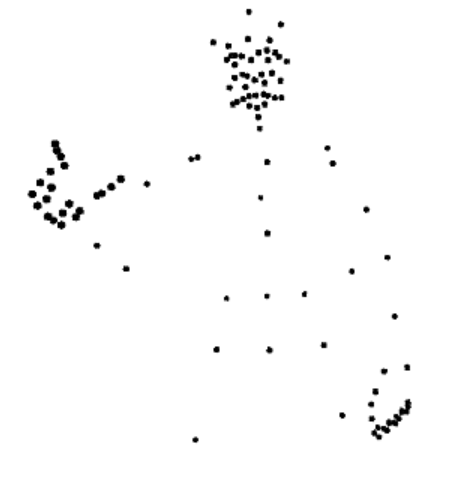
\includegraphics[width=0.34\linewidth]{Images/Johansson.png}
    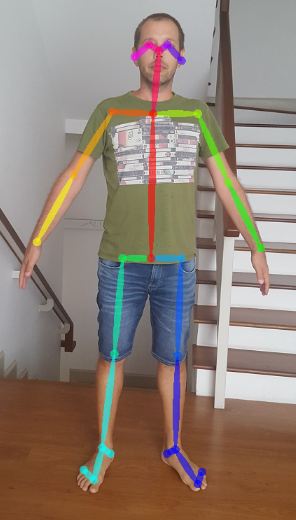
\includegraphics[width=0.2\linewidth]{Images/openpose2.png}
    \caption{A gauche: Un exemple de stimuli de l'experience de Johansson \cite{johansson1973visual,johansson1976spatio}.\\ A droite: la squelettisation obtenue après l'application d'Openpose \cite{cao2017realtime}}
    \label{fig:Johansson}
\end{figure}

Par conséquent, nous 

\textit{De ce fait, nous avons du nous intérésser à plusieurs étapes qui seront considérées comme des parties indépendantes de notre approche}


PipeLine: SQUELETTE -> HAR -> INTENTION

\subsection{Squelettisation de piétons}
La nécéssité première de cette thèse consiste donc en l'obtention d'une squelettisation cohérente de chaque piéton présent dans l'image au fil du temps.

Cette squelettisation sera ensuite utilisée en tant que donnée d'entrée de notre réseau afin d'en inférer une classe en fonction de la gestuelle de celui-ci.

La tâche de détection est compliquée par la variabilité de l’apparence des personnes (vêtements, pose ...)
ainsi que par des phénomènes d’occlusions, dûs à la foule et au décor ou encore dûs à des problèmes d'echelle dans l'image.




\label{subsec:SQUEL}
\subsubsection{Approches Top Down}
\subsubsection{Approches Bottom Up}

\subsection{Human Action Recognition}

\textbf{ Compared to RGB videos and optic flow,skeleton sequences are computationally efficient. Furthermore,skeleton  sequences  have  a  better  ability  to  represent  dataset-invariant  action  information  since  no  background  context  isincluded.
Parler des handcrafted?}

\textit{3D action recognition – analysis of human actions based on3D  skeleton  data  –  becomes  popular  recently  due  to  its  succinctness,robustness, and view-invariant representation}

La seconde étape de l'approche consistera en la classification des actions de la personne,

Les principales modalités utilisées pour la reconnaissance d'actions humaines comprennent les vidéos RGB dans leur globalité \cite{donahue2015long,2014arXiv1412.0767T,varol2017long,Wu_2018_CVPR}, le flow optique \cite{simonyan2014two,zhang2016real,sevilla2018integration,DanutPOP} et la réprésentation sous forme de squelette \cite{vemulapalli2014human,du2015hierarchical,2016arXiv160707043L,2018arXiv180107455Y}.

En réduisant la taille des données d'entrée grâce à la structure de données associée aux squelettes, ce type d'approche est considéré comme bien plus rapide computationellement parlant.

\label{subsec:HAR}

\subsubsection{Image-Based}
\subsubsection{Recurent neural network based}
\subsubsection{Graph Based}

\subsection{Intention Prediction}
\textit{La plupart des approches actuelles de la prédiction de l'action des piétons sont basées sur la trajectoire [16, 1, 5], ce qui signifie qu'elles s'appuient sur le mouvement passé observé des piétons et/ou la dynamique des véhicules pour prédire l'emplacement futur des piétons. Ces approches sont toutefois efficaces lorsque les piétons traversent déjà laa rue ou sont sur le point de le faire, c'est-à-dire que ces algorithmes réagissent à une action déjà en cours au lieu de l'anticiper.}

Un remède aux inconvénients courants des algorithmes basés sur la trajectoire est d'anticiper l'action en estimant sa cause ou son intention non déviante.


In the literature various terms such as intention, actionand behavior are used to describe what the agent is doing or about to do in the scene. Here, we distinguish intention as the underlying state of mind which cannot be observed but can be inferred from the behavior. This is opposed toactions and, more generally, behaviors, i.e. observable ac-tions such as walking or crossing, for which there is groundtruth available.




\subsubsection{Handcrafted}
\subsubsection{Apprentissage profond}




% SEC1
\input{./Sections/Section_2}


%%%%%%%%%%%%%%%%%%%%%%%%%%%%%%%%%%%%%%%%%%%%%%%%%%%%%%%%%%%%%
%APPENDICES
%%%%%%%%%%%%%%%%%%%%%%%%%%%%%%%%%%%%%%%%%%%%%%%%%%%%%%%%%%%%%


\appendix
\renewcommand*{\thesection}{\Alph{section}}\textbf{}

% APPENDIX A
\clearpage
\section{Appendix}
\label{app:A}






%%%%%%%%%%%%%%%%%%%%%%%%%%%%%%%%%%%%%%%%%%%%%%%%%%%%%%%%%%%%%
%BIBLIOGRAPHY
%%%%%%%%%%%%%%%%%%%%%%%%%%%%%%%%%%%%%%%%%%%%%%%%%%%%%%%%%%%%%

\clearpage
\renewcommand*{\thesection}{}\textbf{}

\bibliographystyle{apacite}
\bibliography{Bibliography.bib}


\end{document}